
\documentclass[tikz,border=6pt]{standalone}
\usepackage{amsmath}
\usetikzlibrary{calc}

\begin{document}
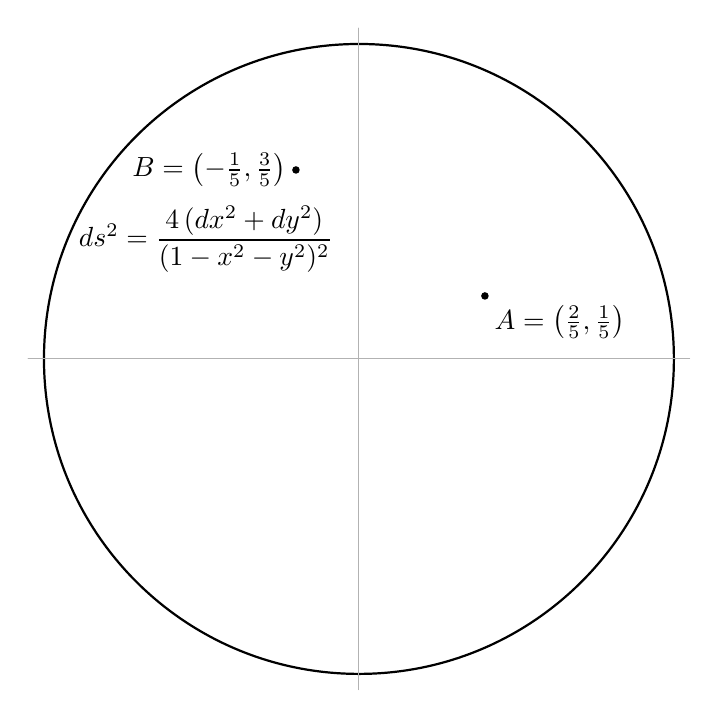
\begin{tikzpicture}[scale=4, line cap=round, line join=round]
  % Unit circle (boundary of the Poincaré disk)
  \draw[thick] (0,0) circle (1);

  % Axes (light gray)
  \draw[gray!60] (-1.05,0) -- (1.05,0);
  \draw[gray!60] (0,-1.05) -- (0,1.05);

  % Metric text inside the disk
  \node[anchor=west] at (-0.92,0.38) {$ds^2=\dfrac{4\,(dx^2+dy^2)}{(1-x^2-y^2)^2}$};

  % Points A and B (asymmetric)
  \coordinate (A) at (0.4,0.2);   % (2/5, 1/5)
  \coordinate (B) at (-0.2,0.6);  % (-1/5, 3/5)

  % Draw points
  \fill (A) circle (0.012);
  \fill (B) circle (0.012);

  % Labels with exact coordinates
  \node[below right] at (A) {$A=\bigl(\tfrac{2}{5},\tfrac{1}{5}\bigr)$};
  \node[left]       at (B) {$B=\bigl(-\tfrac{1}{5},\tfrac{3}{5}\bigr)$};

\end{tikzpicture}
\end{document}
